\documentclass[12pt, a4paper]{article}
\usepackage[utf8]{inputenc}
\usepackage[T1]{fontenc}
\usepackage[french]{babel}
\usepackage{graphicx}
\usepackage[margin=2.5cm]{geometry}
\usepackage{xcolor}
\usepackage{titlesec}
\usepackage{fancyhdr}
\usepackage{enumitem}
\usepackage{booktabs}
\usepackage{amsmath}
\usepackage{array}
\usepackage{colortbl}
\usepackage{hyperref}
\usepackage{microtype}
\usepackage{parskip}

% ===== COULEURS =====
\definecolor{bleuUIDT}{RGB}{0, 51, 102}
\definecolor{bleuClair}{RGB}{0, 102, 204}
\definecolor{grisLeger}{RGB}{245, 245, 245}

% ===== STYLE DES TITRES =====
\titleformat{\section}
  {\normalfont\Large\bfseries\color{bleuUIDT}}
  {\thesection}{1em}{}[\color{bleuClair}\titlerule]
\titleformat{\subsection}
  {\normalfont\large\bfseries\color{bleuClair}}
  {\thesubsection}{1em}{}
\titleformat{\subsubsection}
  {\normalfont\normalsize\bfseries\color{black!80}}
  {\thesubsubsection}{1em}{}
\titlespacing{\section}{0pt}{20pt}{10pt}
\titlespacing{\subsection}{0pt}{15pt}{8pt}

% ===== EN-TÊTE ET PIED DE PAGE =====
\pagestyle{fancy}
\fancyhf{}
\fancyhead[L]{\textcolor{bleuUIDT}{\textbf{UIDT --- LMI 2}}}
\fancyhead[R]{\textcolor{bleuUIDT}{Algorithmique \& Structures de Données}}
\fancyfoot[L]{\textcolor{gray}{\small Ndiaye \& Faye --- 2025-2026}}
\fancyfoot[C]{\textcolor{gray}{\small ---~\thepage~---}}
\fancyfoot[R]{\textcolor{gray}{\small Gestion de Dossiers Médicaux}}
\renewcommand{\headrulewidth}{0.8pt}
\renewcommand{\footrulewidth}{0.4pt}

% ===== HYPERLIENS =====
\hypersetup{
    colorlinks=true,
    linkcolor=bleuUIDT,
    urlcolor=bleuClair,
}

\begin{document}

% ===== PAGE DE TITRE =====
\begin{titlepage}
    \pagecolor{bleuUIDT}
    \color{white}
    \centering
    \vspace*{1.5cm}
    {\large\bfseries République du Sénégal}\\[0.3cm]
    {\large Université Iba Der Thiam de Thiès}\\[0.3cm]
    {\large UFR Sciences et Technologies}\\[0.2cm]
    {\large Département de Mathématiques et Informatique}\\[2cm]
    \noindent\rule{\textwidth}{0.5pt}\\[0.5cm]
    {\Huge\bfseries Conception et Implémentation\\[0.3cm]
    de Structures de Données}\\[0.3cm]
    \noindent\rule{\textwidth}{0.5pt}\\[0.5cm]
    {\Large pour un Système de Gestion\\[0.2cm]
    de Dossiers Médicaux}\\[2.5cm]
    \begin{minipage}{0.45\textwidth}
        \centering
        {\large\bfseries Réalisé par :}\\[0.3cm]
        {\Large Coumba \textsc{Ndiaye}}\\[0.2cm]
        {\Large Moussa \textsc{Faye}}
    \end{minipage}
    \hfill
    \begin{minipage}{0.45\textwidth}
        \centering
        {\large\bfseries Encadrant :}\\[0.3cm]
        {\Large Dr Abdoulaye \textsc{Diallo}}
    \end{minipage}
    \vfill
    {\large Licence 2 Mathématiques-Informatique}\\[0.3cm]
    {\large Année universitaire 2025--2026}
\end{titlepage}
\pagecolor{white}
\color{black}

\newpage
\tableofcontents
\newpage

% ===== INTRODUCTION =====
\section{Introduction}

Dans tout système informatique, le choix des structures de données 
conditionne directement la performance des opérations fondamentales. 
Ce projet s'inscrit dans le cadre du cours d'\textbf{Algorithmique 
et Structures de Données} de la Licence 2 Mathématiques-Informatique 
de l'Université Iba Der Thiam de Thiès.

Nous avons choisi le domaine de la \textbf{gestion de dossiers médicaux}, 
qui consiste à gérer les informations des patients et leurs consultations 
dans un centre de santé.

L'objectif principal est d'implémenter et de comparer trois structures 
de données en langage C :
\begin{itemize}[leftmargin=2em, itemsep=3pt]
    \item Le \textbf{tableau statique} : structure simple à taille fixe
    \item Le \textbf{tableau dynamique} : structure à redimensionnement automatique
    \item La \textbf{liste chaînée} : structure à allocation dynamique par nœud
\end{itemize}

Ce rapport présente la modélisation des données, l'implémentation 
des structures, une analyse de complexité théorique, et une étude 
expérimentale comparative appuyée par des courbes scientifiques.

% ===== MODÉLISATION =====
\section{Modélisation des données}

\subsection{Structure Patient}

\begin{table}[h]
\centering
\rowcolors{2}{grisLeger}{white}
\begin{tabular}{>{\ttfamily}l l}
\toprule
\textbf{Champ} & \textbf{Description} \\
\midrule
int id & Identifiant unique (clé primaire) \\
char prenom[25] & Prénom du patient \\
char nom[25] & Nom de famille \\
char sexe & Sexe (M ou F) \\
char adresse[50] & Adresse complète \\
char numTel[15] & Numéro de téléphone \\
int age & Âge en années \\
Date date\_naissance & Date de naissance \\
float poids & Poids en kilogrammes \\
float taille & Taille en mètres \\
struct consultation* consultations & Pointeur vers les consultations \\
int nb\_consultations & Nombre de consultations \\
\bottomrule
\end{tabular}
\caption{Champs de la structure \texttt{patient}}
\end{table}

\subsection{Structure Consultation}

\begin{table}[h]
\centering
\rowcolors{2}{grisLeger}{white}
\begin{tabular}{>{\ttfamily}l l}
\toprule
\textbf{Champ} & \textbf{Description} \\
\midrule
int id & Identifiant unique \\
Date date\_consultation & Date de la consultation \\
char medecin[25] & Nom du médecin \\
char diagnostic[100] & Diagnostic établi \\
char traitement[100] & Traitement prescrit \\
int duree & Durée en jours \\
float cout & Coût en FCFA \\
struct patient* patient & Pointeur vers le patient \\
\bottomrule
\end{tabular}
\caption{Champs de la structure \texttt{consultation}}
\end{table}

\subsection{Relation entre les structures}
Les deux structures sont liées par des pointeurs, formant une 
relation \textbf{1-N} : un patient peut avoir plusieurs consultations, 
et chaque consultation référence son patient.

% ===== STRUCTURES =====
\section{Structures de données implémentées}

\subsection{Tableau statique}
Tableau de taille fixe défini à la compilation, pouvant contenir 
au maximum \textbf{100 patients}.

\subsubsection{Caractéristiques}
\begin{itemize}[leftmargin=2em, itemsep=3pt]
    \item Taille fixe de 100 éléments
    \item Accès direct par indice en $O(1)$
    \item Aucune gestion dynamique de la mémoire
\end{itemize}

\subsubsection{Opérations}
\begin{itemize}[leftmargin=2em, itemsep=3pt]
    \item \textbf{Insertion} : ajout à la position \texttt{taille}
    \item \textbf{Recherche par clé} : parcours séquentiel
    \item \textbf{Recherche par intervalle} : patients entre deux âges
    \item \textbf{Recherche par préfixe} : patients par début de nom
    \item \textbf{Suppression} : remplacement par le dernier élément
    \item \textbf{Modification} : mise à jour par identifiant
    \item \textbf{Tri par insertion} : tri alphabétique sur le nom
    \item \textbf{Tri rapide} : tri numérique sur l'âge
    \item \textbf{Agrégations} : min, max, moyenne, médiane, écart-type
    \item \textbf{Persistance} : sauvegarde et chargement binaire
\end{itemize}

\subsection{Tableau dynamique}
Utilise \texttt{malloc} et \texttt{realloc}. La capacité 
\textbf{double automatiquement} lorsqu'elle est atteinte.

\subsubsection{Principe du redimensionnement}
\begin{verbatim}
if (*taille >= *capacite) {
    *capacite *= 2;
    *tableau = realloc(*tableau, (*capacite) * sizeof(patient));
}
\end{verbatim}

\subsubsection{Caractéristiques}
\begin{itemize}[leftmargin=2em, itemsep=3pt]
    \item Capacité initiale de 2 éléments
    \item Facteur de croissance géométrique de 2
    \item Accès direct par indice en $O(1)$
    \item Libération mémoire avec \texttt{free()}
\end{itemize}

\subsection{Liste chaînée}
Structure où chaque nœud contient les données et un pointeur 
vers le nœud suivant.

\subsubsection{Structure d'un nœud}
\begin{verbatim}
typedef struct Noeud {
    patient data;
    struct Noeud* suivant;
} Noeud;

typedef struct {
    Noeud* tete;
    int taille;
} ListeChainee;
\end{verbatim}

\subsubsection{Caractéristiques}
\begin{itemize}[leftmargin=2em, itemsep=3pt]
    \item Insertion en tête en $O(1)$
    \item Insertion en queue en $O(n)$
    \item Aucune limite de taille
    \item Allocation mémoire individuelle par nœud
\end{itemize}

% ===== COMPLEXITÉ =====
\section{Analyse de complexité}

\subsection{Tableau récapitulatif}

\begin{table}[h]
\centering
\rowcolors{2}{grisLeger}{white}
\begin{tabular}{l c c c}
\toprule
\textbf{Opération} & \textbf{Tableau statique} & \textbf{Tableau dynamique} & \textbf{Liste chaînée} \\
\midrule
Insertion & $O(1)$ & $O(1)$ amorti & $O(1)$ tête \\
Recherche par clé & $O(n)$ & $O(n)$ & $O(n)$ \\
Suppression & $O(n)$ & $O(n)$ & $O(n)$ \\
Modification & $O(n)$ & $O(n)$ & $O(n)$ \\
Tri par insertion & $O(n^2)$ & $O(n^2)$ & $O(n^2)$ \\
Tri rapide & $O(n\log n)$ & $O(n\log n)$ & --- \\
Agrégations & $O(n)$ & $O(n)$ & $O(n)$ \\
\midrule
\textbf{Espace} & $\Theta(1)$ fixe & $\Theta(n)$ & $\Theta(n)$ + pointeurs \\
\bottomrule
\end{tabular}
\caption{Complexités des trois structures}
\end{table}

\subsection{Justifications mathématiques}

\textbf{Insertion en $O(1)$} : L'ajout se fait directement à la 
position \texttt{taille} sans décalage. Pour le tableau dynamique, 
le coût amorti reste $O(1)$ car le doublement ne survient qu'en 
$O(\log n)$ occasions sur $n$ insertions.

\textbf{Tri par insertion en $O(n^2)$} :
$$\sum_{i=1}^{n-1} i = \frac{n(n-1)}{2} = \Theta(n^2)$$
Dans le meilleur cas (tableau déjà trié) : $\Omega(n)$.

\textbf{Tri rapide en $O(n\log n)$} :
$$T(n) = 2T\left(\frac{n}{2}\right) + \Theta(n) \Rightarrow \Theta(n\log n)$$
Dans le pire cas : $O(n^2)$.

\subsection{Discussion}
Pour le tri rapide, le choix du dernier élément comme pivot 
conduit au pire cas $O(n^2)$ sur des données déjà triées. 
Sur des données uniformément distribuées, le comportement 
moyen $\Theta(n\log n)$ est observé.

% ===== ÉTUDE EXPÉRIMENTALE =====
\section{Étude expérimentale}

\subsection{Protocole expérimental}

\begin{table}[h]
\centering
\rowcolors{2}{grisLeger}{white}
\begin{tabular}{l l}
\toprule
\textbf{Paramètre} & \textbf{Valeur} \\
\midrule
Système d'exploitation & Windows 11 \\
Compilateur & GCC 16.1 (MinGW) \\
Répétitions par mesure & 10 \\
Tailles (statique) & n = 10, 50, 100 \\
Tailles (dynamique \& liste) & n = 100, 1\,000, 10\,000 \\
\bottomrule
\end{tabular}
\caption{Conditions expérimentales}
\end{table}

\subsection{Temps d'insertion}

\begin{figure}[h]
    \centering
    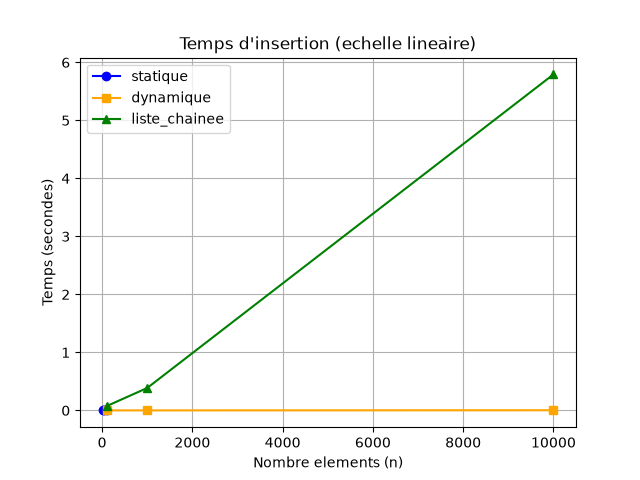
\includegraphics[width=0.85\textwidth]{courbe_insertion_lineaire.png}
    \caption{Temps d'insertion en échelle linéaire}
\end{figure}

\begin{figure}[h]
    \centering
    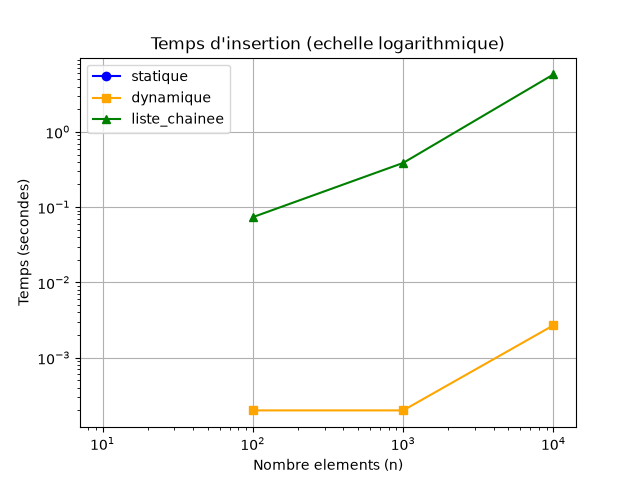
\includegraphics[width=0.85\textwidth]{courbe_insertion_log.png}
    \caption{Temps d'insertion en échelle logarithmique}
\end{figure}

La liste chaînée est plus lente que les tableaux pour l'insertion, 
en raison de l'appel à \texttt{malloc} pour chaque nœud.

\subsection{Temps de recherche}

\begin{figure}[h]
    \centering
    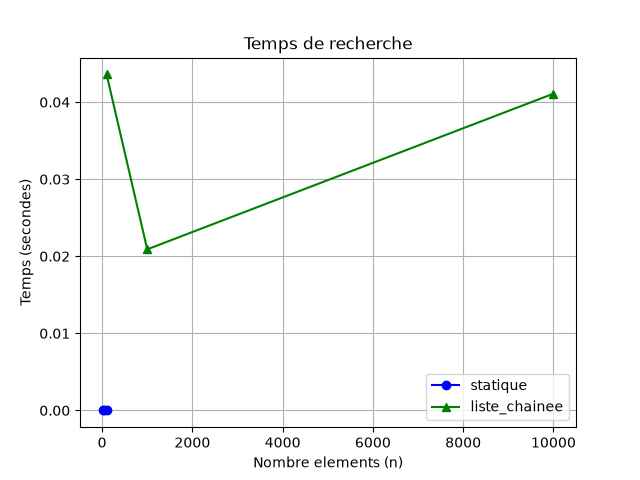
\includegraphics[width=0.85\textwidth]{courbe_recherche.png}
    \caption{Temps de recherche par clé pour chaque structure}
\end{figure}

\subsection{Temps de tri}

\begin{figure}[h]
    \centering
    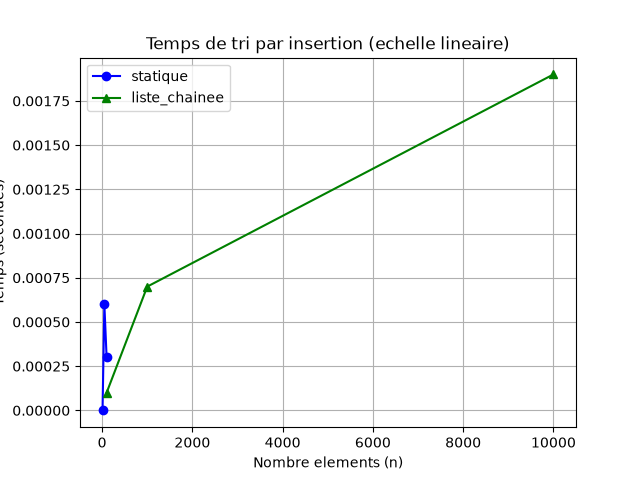
\includegraphics[width=0.85\textwidth]{courbe_tri_insertion_lineaire.png}
    \caption{Temps de tri par insertion en échelle linéaire}
\end{figure}

\begin{figure}[h]
    \centering
    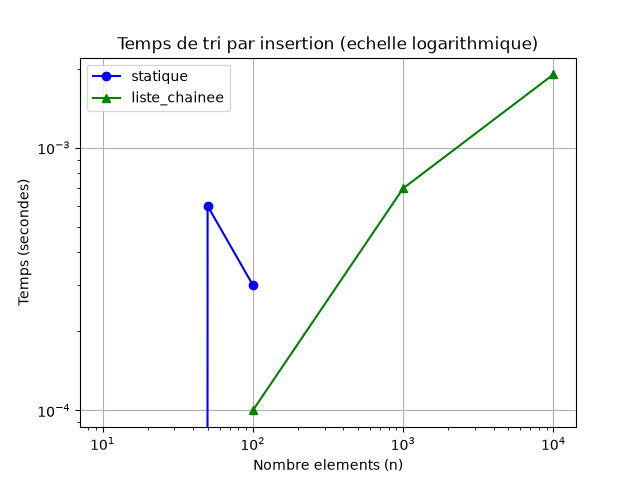
\includegraphics[width=0.85\textwidth]{courbe_tri_insertion_log.png}
    \caption{Temps de tri par insertion en échelle logarithmique}
\end{figure}

\begin{figure}[h]
    \centering
    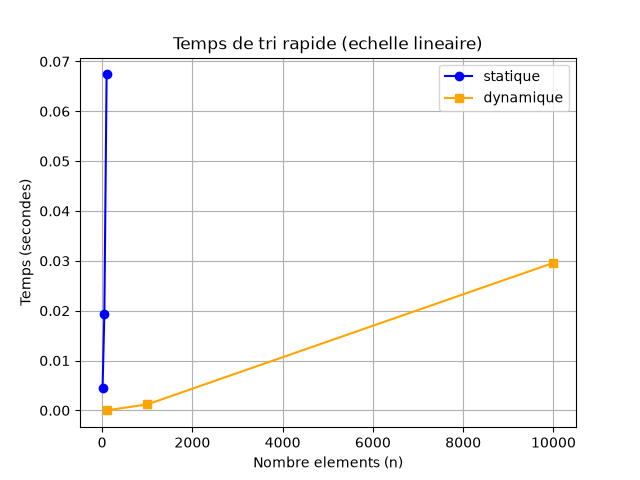
\includegraphics[width=0.85\textwidth]{courbe_tri_rapide_lineaire.png}
    \caption{Temps de tri rapide en échelle linéaire}
\end{figure}

\subsection{Courbe théorique vs empirique}

\begin{figure}[h]
    \centering
    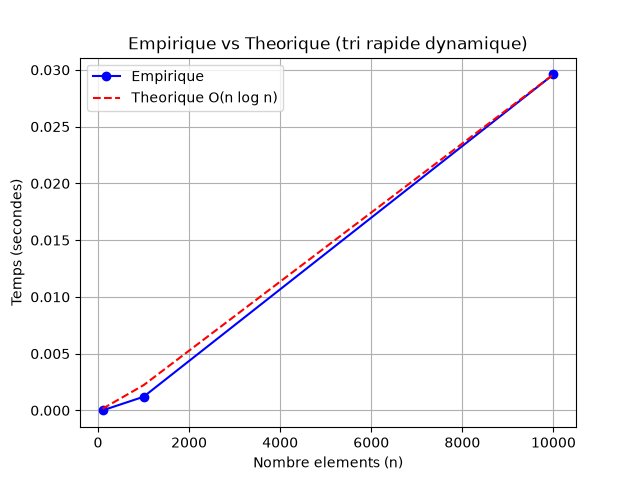
\includegraphics[width=0.85\textwidth]{courbe_theorique_vs_empirique.png}
    \caption{Courbe empirique vs théorique $O(n\log n)$}
\end{figure}

La courbe empirique suit bien la courbe théorique $O(n\log n)$, 
confirmant notre analyse de complexité.

\subsection{Comparaison globale}

\begin{figure}[h]
    \centering
    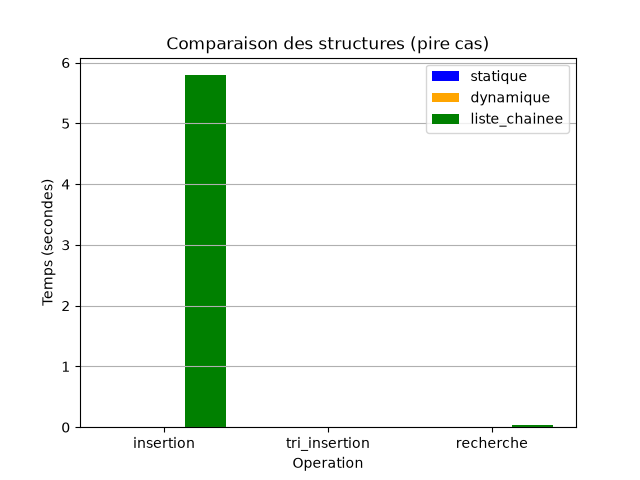
\includegraphics[width=0.85\textwidth]{courbe_histogramme.png}
    \caption{Histogramme comparatif des trois structures}
\end{figure}

L'histogramme confirme que la liste chaînée est la structure la 
plus lente. Le tableau dynamique et le tableau statique présentent 
des performances comparables.

% ===== CONCLUSION =====
\section{Conclusion}

Ce projet nous a permis de mettre en pratique les notions 
fondamentales de l'algorithmique et des structures de données 
à travers un cas concret de gestion de dossiers médicaux.

Les principaux enseignements sont :
\begin{itemize}[leftmargin=2em, itemsep=5pt]
    \item Le \textbf{tableau statique} est le plus rapide pour 
    les petits volumes, mais limité à 100 éléments.
    \item Le \textbf{tableau dynamique} offre le meilleur 
    compromis entre performance et flexibilité.
    \item La \textbf{liste chaînée} offre une insertion en tête 
    en $O(1)$ et une taille illimitée, au prix d'une performance 
    moindre en pratique.
\end{itemize}

Ce travail nous a permis de renforcer notre maîtrise des 
\textbf{pointeurs en C}, de la \textbf{gestion mémoire dynamique}, 
et des outils professionnels tels que Git, GCC et Python.

\begin{thebibliography}{9}
\bibitem{cormen}
Cormen T. H. et al.,
\textit{Introduction to Algorithms},
4\textsuperscript{e} édition, MIT Press, 2022.

\bibitem{kernighan}
Kernighan B. W., Ritchie D. M.,
\textit{The C Programming Language},
2\textsuperscript{e} édition, Prentice Hall.

\bibitem{sedgewick}
Sedgewick R., Wayne K.,
\textit{Algorithms}, 4\textsuperscript{e} édition,
Addison-Wesley, 2011.

\bibitem{beauquier}
Beauquier D., Berstel J., Chrétienne P.,
\textit{Éléments d'algorithmique}, Masson.
\end{thebibliography}

\end{document}